\documentclass[oneside,14pt]{extarticle}
\usepackage[utf8]{inputenc}
\usepackage[english,ukrainian]{babel}
\usepackage{amssymb,amsfonts,amsmath,amsthm,mathtext,textcomp}

\usepackage[includehead, headsep=0pt, footskip=0pt, top=2cm, bottom=2cm, left=2cm, right=1cm]{geometry}
\usepackage{indentfirst}
\usepackage[onehalfspacing]{setspace}
\usepackage[headings]{fancyhdr}
\usepackage{etoolbox}
\usepackage{flafter}
\usepackage{listings}
\usepackage{graphicx}
\usepackage{float}
\usepackage[center]{titlesec}
\titlelabel{\thetitle.\quad}
\usepackage{array}
\fancyhf{}
\renewcommand{\headrulewidth}{0pt}
\pagestyle{fancy}
\fancyfoot[R]{\thepage}
\lstset{breaklines=true,}
\graphicspath{ {./pictures} }
\counterwithin{figure}{section}

\begin{document}
\begin{titlepage}
	\begin{center}
		Національний університет “Львівська політехніка”\\
		Кафедра програмного забезпечення
		
		\vspace{170pt}
		\textbf{КУРСОВА РОБОТА}\\
		\textbf{з дисципліни <<Об’єктно-орієнтоване програмування>>}\\
		\textbf{На тему:}\\
		<<Медична база пацієнтів>>
		\vspace*{40pt}
		
		\begin{flushright}
			Стедента групи ПЗ-22\\
			спеціальності 6.121\\
			“Програмна інженерія”\\
			Коваленко Д.М.
			\bigbreak
			
			Керівник: доцент кафедри ПЗ,\\
			к.т.н., доцент Коротєєва Т. О.
			\bigbreak
			
			Національна шкала \rule{4cm}{0.15mm}\\			
			Кількість \rule{1cm}{0.15mm} балів  Оцінка ECTS \rule{1cm}{0.15mm}
			\bigbreak
			
			Члени комісії \rule{1cm}{0.15mm} \rule{4cm}{0.15mm}\\
			\rule{1cm}{0.15mm} \rule{4cm}{0.15mm}\\
			\rule{1cm}{0.15mm} \rule{4cm}{0.15mm}
		\end{flushright}
		\vspace{\fill}
		Львів — 2022
	\end{center}
\end{titlepage}
\setcounter{page}{2}
\tableofcontents
\newpage
\section*{Завдання}
\addcontentsline{toc}{section}{Завдання}
\begin{center}
	на курсову роботу з дисципліни «Об’єктно-орієнтоване програмування»\\
	студента групи ПЗ-22 Коваленка Дмитра
	\bigbreak
	\textbf{Тема: <<Медична база пацієнтів>>}
\end{center}
Створити таблицю у візуальному середовищі

\begin{tabular}{|c|c|c|c|c|c|c|}
	\hline
	№ & Прізвище & Вік & Група крові & Резус-фактор & Артеріальний тиск & Пульс\\
	\hline
\end{tabular}

\begin{enumerate}
	\item Швидким алгоритмом відсортувати записи за показником артеріального
	тиску.
	\item Згрупувати людей за однаковими групами крові та однаковими резус
	факторами.
	\item Згрупувати людей за однаковими резус-факторами та відсортувати кожну
	групу за показником Пульсу.
	\item Визначити людей, які є універсальними донорами, а які є універсальними
	реципієнтами та сформувати загальну таблицю донорів та реципієнтів.
	\item Для вказаного показника Вік визначити пацієнтів з підвищеними показниками
	артеріального тиску та пульсу.
	\item Всім пацієнтам з нормальними артеріальним тиском вивести повідомлення
	<<Прізвище --- Здоровий!>>
\end{enumerate}
Для класу створити: 1) Конструктор за замовчуванням; 2) Конструктор з
параметрами; 3) конструктор копій; 4) перевизначити операції $>>$, $<<$ для
зчитування та запису у файл.
\newpage
\begin{center}
	\textbf{Зміст завдання та календарний план його виконання}
	
	\begin{tabular}{ | m{0.7cm} | m{14cm}| m{1.1cm} | }
		\hline
		№ з/п & Зміст завдання & Дата \\ 
		\hline
		1 & Здійснити аналiтичний огляд лiтератури за заданою темою та обгрунтувати вибір інструментальних засобів реалізації. & 09.10 \\
		\hline
		2 & Побудова UML діаграм & 10.10 \\
		\hline
		3 & Розробка алгоритмів реалізації & 13.10 \\
		\hline
		4 & Реалізація завдання (кодування) & 15.10 \\
		\hline
		5 & Формування інструкції користувача & 17.10 \\
		\hline
		6 & Оформлення звіту до курсової роботи згідно з вимогами Міжнародних стандартів, дотримуючись такої структури:
		
		·       зміст;
		
		·       алгоритм розв‘язку задачі у покроковому представленні;
		
		·       діаграми UML класів, прецедентів, послідовності виконання;
		
		·       код розробленої програми з коментарями;
		
		·       протокол роботи програми для кожного пункту завдання
		
		·       інструкція користувача та системні вимоги;
		
		·       опис виняткових ситуацій;
		
		·       структура файлу вхідних даних;
		
		·       висновки;
		
		·       список використаних джерел. & 18.10 \\
		\hline
	\end{tabular}
\end{center}
Завдання прийнято до виконання: \rule{4cm}{0.15mm} Коваленко Д.М.\\
Керівник роботи: \rule{4cm}{0.15mm} Коротєєва Т. О.

\section{Покроковий алгоритм розв‘язку задачі}
\subsection{Задача сортування}
\begin{list}{}{Алгоритм A.}
	\item [A1] Виклик функції сортування користувачем.
	\item [A2] Сортування списку за заданим стовпцем.
	\item [A3] Виведення посортованого списку на екран.
	\item [A4] Кінець.
\end{list}

\subsection{Задача групування}
\begin{list}{}{Алгоритм B.}
	\item [B1] Вибір користувачем стовпця, за яким необхідно згрупувати список.
	\item [B2] Сортування списку за заданим стовпцем.
	\item [B3] Виведення згрупованого списку на екран.
	\item [B4] Кінець.
\end{list}

\subsection{Згрупувати людей та відсортувати кожну групу}
\begin{list}{}{Алгоритм C.}
	\item [C1] Виклик функції сортування користувачем.
	\item [C2] Сортування списку за двома умовами одночасно.
	\item [C3] Виведення посортованого списку на екран.
	\item [C4] Кінець.
\end{list}

\subsection{Задача визначити групи людей зі списку за умовою}
\begin{list}{}{Алгоритм D.}
	\item [D1] Вибір користувачем групи яку необхідно визначити.
	\item [D2] Виведення на екран людей, дані яких задовільняють умову.
	\item [D3] Кінець.
\end{list}

\subsection{Задача визначети людей за вказаними даними}
\begin{list}{}{Алгоритм E.}
	\item [E1] Ввід користувачем необхідних даних.
	\item [E2] Виведення на екран пацієнтів, дані яких задовільняють умову.
	\item [E3] Кінець.
\end{list}

\subsection{Задача виведення повідомлення}
\begin{list}{}{Алгоритм F.}
	\item [F1] Визначення пацієнтів, дані яких задовільняють умову.
	\item [F2] Виведення на екран повідомлення для кожного пацієнта. 
	\item [F3] Кінець.
\end{list}

\section{Діаграми}
\subsection{UML діаграма класів}
\begin{figure}[H]
	\centering
	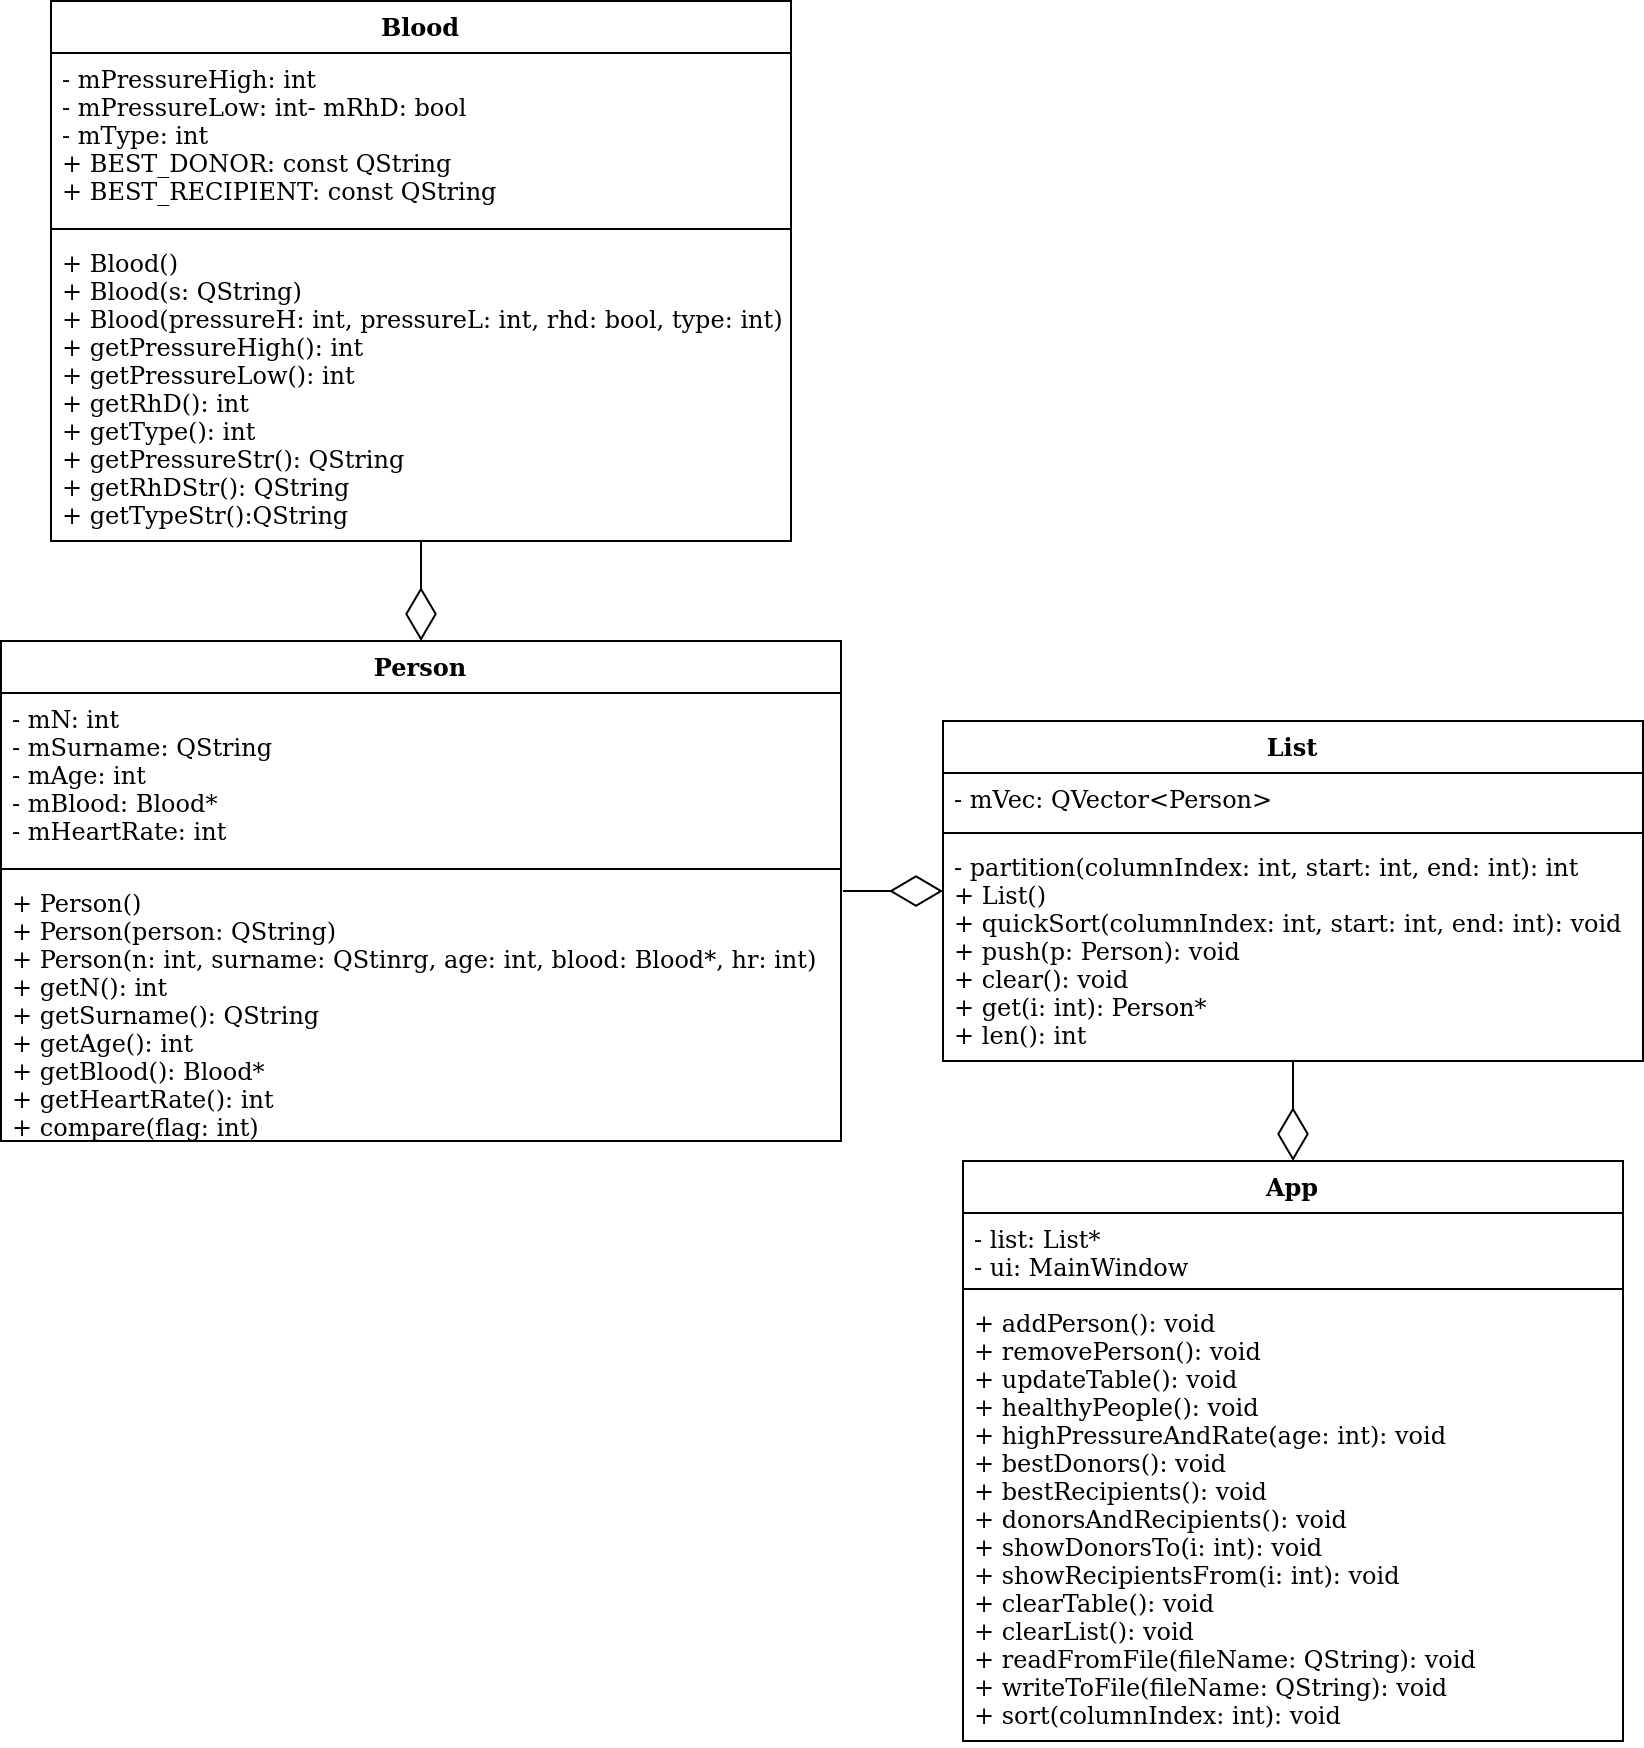
\includegraphics[scale=0.3]{1}
	\caption{UML діаграма класів}
\end{figure}

\subsection{Діаграма прецедентів}
\begin{figure}[H]
	\centering
	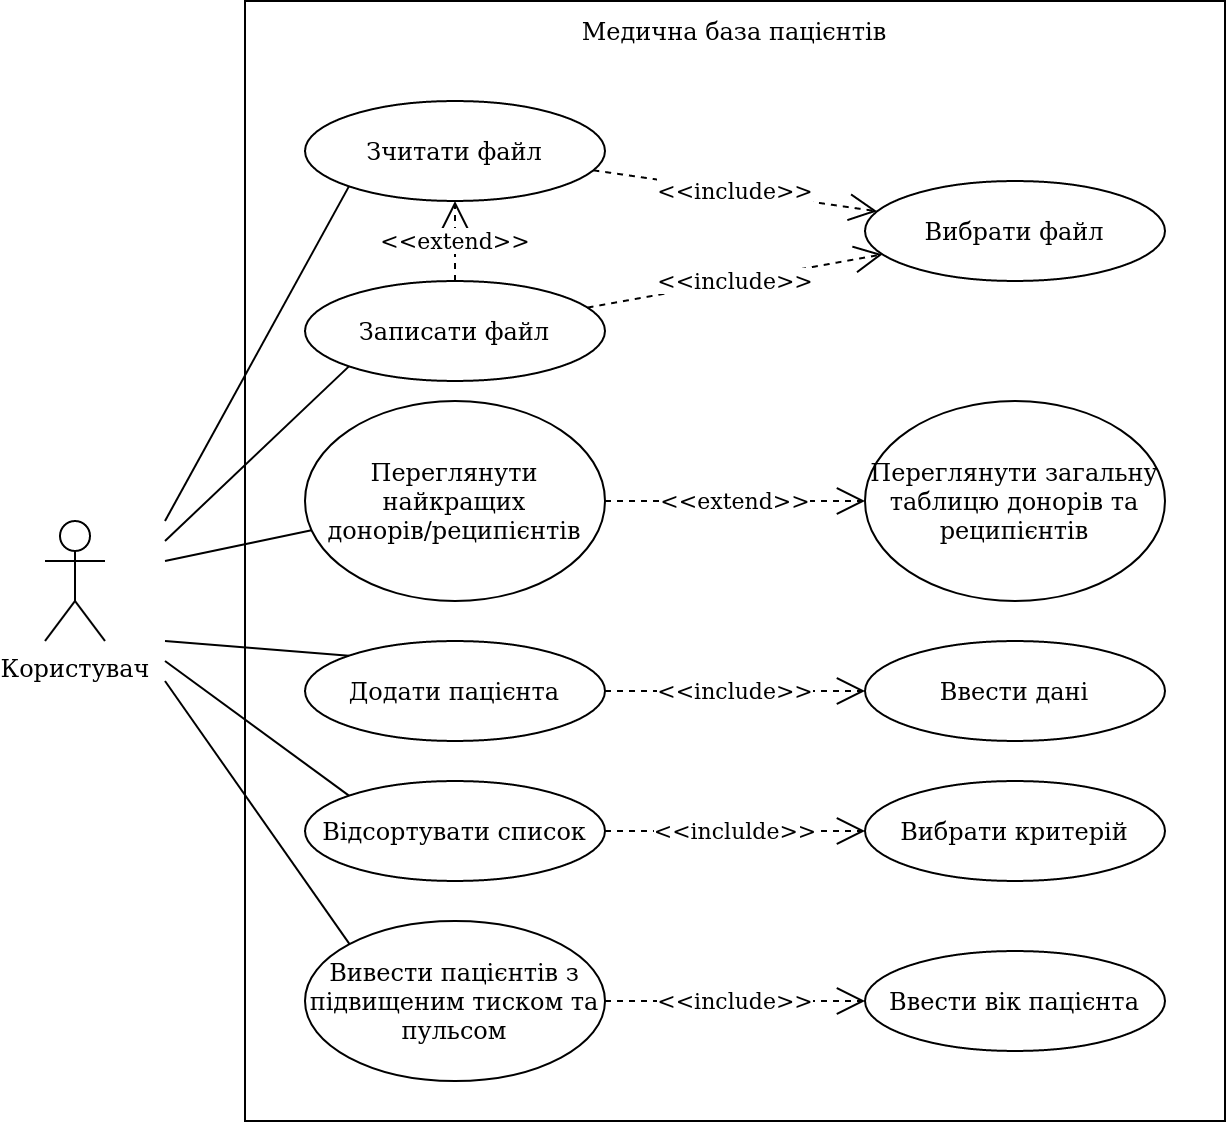
\includegraphics[scale=0.4]{2}
	\caption{Діаграма прецедентів}
\end{figure}

\subsection{Діаграма послідовності виконання}
\begin{figure}[H]
	\centering
	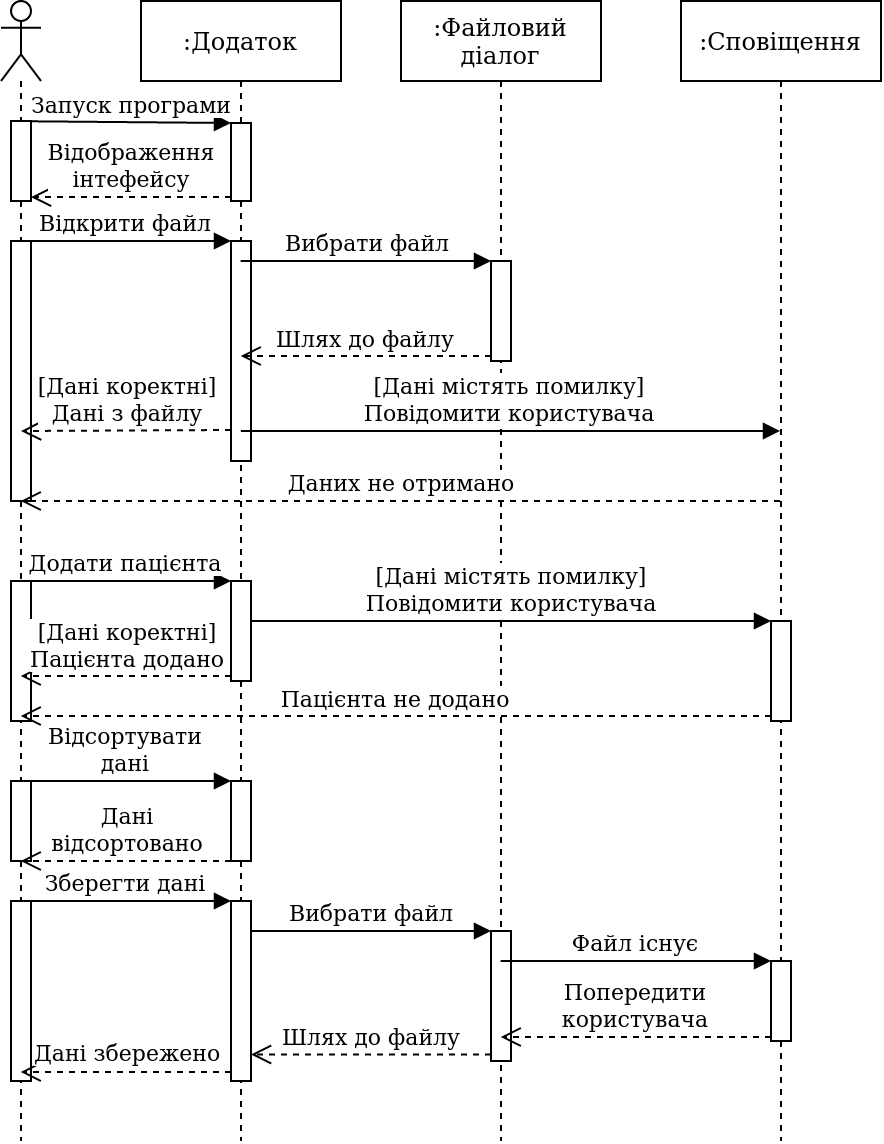
\includegraphics[scale=0.5]{3}
	\caption{Діаграма послідовності виконання}
\end{figure}

\section{Код розробленої програми}
\begin{small}
\textbf{файл \textit{app.h}}
\begin{lstlisting}[language=c++]
#ifndef APP_H
#define APP_H

#include "list.h"
#include "mainwindow.h"
#include "ui_mainwindow.h"

class App
{
	private:
	List* list;
	Ui::MainWindow* ui;
	
	public:
	App() = default;
	App(Ui::MainWindow* ui);
	
	void addPerson();
	void removePerson();
	void updateTable();
	void healthyPeople();
	void highPressureAndRate(int age);
	void bestDonors();
	void bestRecipients();
	void donorsAndRecipients();
	void showDonorsTo(int i);
	void showRecipientsFrom(int i);
	void clearTable();
	void clearList();
	void readFromFile(QString fileName);
	void writeToFile(QString fileName);
	void sort(int columnIndex);
	
};

#endif // APP_H
\end{lstlisting}

\textbf{файл \textit{blood.h}}
\begin{lstlisting}[language=c++]
#ifndef BLOOD_H
#define BLOOD_H

#include "QString"

class Blood
{
	private:
	int mPressureHigh;
	int mPressureLow;
	bool mRhD;
	int mType;
	
	public:
	const QString BEST_DONOR = "O";
	const QString BEST_RECIPIENT = "AB";
	
	Blood() = default;
	Blood(QString s);
	Blood(int pressureH, int pressureL, bool rhd, int type);
	
	int     getPressureHigh()   const { return this->mPressureHigh; }
	int     getPressureLow()    const { return this->mPressureLow; }
	bool    getRhD()            const { return this->mRhD; }
	int     getType()           const { return this->mType; }
	
	QString getPressureStr();
	QString getRhDStr();
	QString getTypeStr();
	
	bool operator > (const Blood& other) const { return this->mPressureLow + this->mPressureHigh > other.mPressureHigh + other.mPressureLow; }
	bool operator < (const Blood& other) const { return this->mPressureLow + this->mPressureHigh < other.mPressureHigh + other.mPressureLow; }
};

#endif // BLOOD_H
\end{lstlisting}

\textbf{файл \textit{list.h}}
\begin{lstlisting}[language=c++]
#ifndef LIST_H
#define LIST_H

#include "QVector"
#include "QFile"

#include "person.h"

class List
{
	private:
	QVector<Person> mVec;
	int      partition(int columnIndex, int start, int end);
	
	public:
	List() = default;
	
	void     quickSort(int columnIndex, int start, int end);
	void     push(Person p);
	void     clear();
	Person * get(int i);
	int      len() const;
	
	friend void operator << (QFile &output, const List* l);
	friend void operator >> (QFile &input, List* l);
};

#endif // LIST_H
\end{lstlisting}

\textbf{файл \textit{mainwindow.h}}
\begin{lstlisting}[language=c++]
#ifndef MAINWINDOW_H
#define MAINWINDOW_H

#include <QMainWindow>

QT_BEGIN_NAMESPACE
namespace Ui { class MainWindow; }
QT_END_NAMESPACE

class MainWindow : public QMainWindow
{
	Q_OBJECT
	
	public:
	MainWindow(QWidget *parent = nullptr);
	~MainWindow();
	
	private slots:
	void on_actionOpen_triggered();
	void on_actionSave_triggered();
	void on_addPersonBtn_clicked();
	void on_actionby_Blood_Pressure_triggered();
	void on_actionType_and_RhD_triggered();
	void on_actionRhD_and_Heart_Rate_triggered();
	void on_healthyPeople_triggered();
	void on_highPressureAndRate_triggered();
	void on_actionDefault_triggered();
	void on_bestDonors_triggered();
	void on_bestRecipients_triggered();
	void on_donorsRecepients_triggered();
	void on_tableWidget_cellDoubleClicked(int row, int column);
	void on_actionClose_triggered();
	void on_actionRhD_triggered();
	
	private:
	Ui::MainWindow *ui;
};
#endif // MAINWINDOW_H

\end{lstlisting}

\textbf{файл \textit{person.h}}
\begin{lstlisting}[language=c++]
#ifndef PERSON_H
#define PERSON_H

#include "QString"
#include "QTextStream"
#include "blood.h"
#include "QDebug"

class Person
{
	private:
	int     mN;
	QString mSurname;
	int     mAge;
	Blood * mBlood;
	int     mHeartRate;
	
	public:
	Person() = default;
	Person(QString person);
	Person(int n, QString surname, int age, Blood* blood, int hr);
	
	Person(const Person &other);
	
	int     getN()          const { return this->mN;         }
	QString getSurname()    const { return this->mSurname;   }
	int     getAge()        const { return this->mAge;       }
	Blood * getBlood()      const { return this->mBlood;     }
	int     getHeartRate()  const { return this->mHeartRate; }
	
	bool    compare(const Person& other, const int flag) const;
	
	friend void operator << (QTextStream &output, const Person* p);
	friend void operator >> (QTextStream &input, Person* p);
};

#endif // PERSON_H

\end{lstlisting}

\textbf{файл \textit{app.cpp}}
\begin{lstlisting}[language=c++]
#include "app.h"
#include "QDebug"

App::App(Ui::MainWindow* ui)
{
	this->list = new List();
	this->ui = ui;
}

void App::addPerson()
{
	bool ok;
	if (ui->nLE->text().toInt(&ok) == 0)
	if (!ok)
	throw 1;
	if (ui->ageLE->text().toInt(&ok) == 0)
	if (!ok)
	throw 3;
	if (ui->bloodtypeLE->text() != "O" && ui->bloodtypeLE->text() != "A" && ui->bloodtypeLE->text() != "B" && ui->bloodtypeLE->text() != "AB")
	throw 4;
	if (!ui->bloodpressureLE->text().contains("/"))
	throw 5;
	if (ui->rhdLE->text() != "+" && ui->rhdLE->text() != "-")
	throw 6;
	if (ui->heartrateLE->text().toInt(&ok) == 0)
	if (!ok)
	throw 7;
	QString s = ui->nLE->text() + "," +
	ui->surnameLE->text() + "," +
	ui->ageLE->text() + "," +
	ui->bloodpressureLE->text() + " " +
	ui->bloodtypeLE->text() +
	ui->rhdLE->text() + "," +
	ui->heartrateLE->text();
	Person p = Person(s);
	this->list->push(p);
}

void App::updateTable()
{
	ui->tableHealthy->setVisible(false);
	ui->tableWidget->setVisible(true);
	ui->tableDonorsAndRecipients->setVisible(false);
	this->clearTable();
	for (int i = 0; i < list->len(); i++)
	{
		ui->tableWidget->insertRow(i);
		Person * p = this->list->get(i);
		for (int j = 0; j < 7; j++)
		{
			QTableWidgetItem * item = new QTableWidgetItem();
			item->setTextAlignment(Qt::AlignCenter);
			switch (j)
			{
				case 0:
				item->setText(QString::number(p->getN()));
				break;
				case 1:
				item->setText(p->getSurname());
				break;
				case 2:
				item->setText(QString::number(p->getAge()));
				break;
				case 3:
				item->setText(p->getBlood()->getTypeStr());
				break;
				case 4:
				item->setText(p->getBlood()->getRhDStr());
				break;
				case 5:
				item->setText(p->getBlood()->getPressureStr());
				break;
				case 6:
				item->setText(QString::number(p->getHeartRate()));
				break;
			}
			ui->tableWidget->setItem(i, j, item);
		}
	}
}

void App::healthyPeople()
{
	ui->tableHealthy->setVisible(true);
	ui->tableWidget->setVisible(false);
	ui->tableDonorsAndRecipients->setVisible(false);
	ui->tableHealthy->setColumnCount(2);
	ui->tableHealthy->setRowCount(0);
	ui->tableHealthy->setColumnWidth( 0, 360 );
	ui->tableHealthy->setColumnWidth( 1, 360 );
	QStringList labels;
	labels << "Surname" << "Message";
	ui->tableHealthy->setHorizontalHeaderLabels(labels);
	int r = 0;
	for (int i = 0; i < list->len(); i++)
	{
		Person * p = this->list->get(i);
		bool healthy = p->getBlood()->getPressureHigh() <= 140 &&
		p->getBlood()->getPressureLow() <= 100 &&
		p->getBlood()->getPressureHigh() >= 100 &&
		p->getBlood()->getPressureLow() >= 60;
		
		if (healthy)
		ui->tableHealthy->insertRow(r);
		else
		continue;
		for (int j = 0; j < 2; j++)
		{
			QTableWidgetItem * item = new QTableWidgetItem();
			item->setTextAlignment(Qt::AlignCenter);
			switch (j)
			{
				case 0:
				item->setText(p->getSurname());
				break;
				case 1:
				item->setText(QString::fromStdString("Healthy"));
				break;
			}
			ui->tableHealthy->setItem(r, j, item);
		}
		r++;
	}
}

void App::highPressureAndRate(int age)
{
	ui->tableHealthy->setVisible(false);
	ui->tableWidget->setVisible(true);
	ui->tableDonorsAndRecipients->setVisible(false);
	this->clearTable();
	int r = 0;
	for (int i = 0; i < list->len(); i++)
	{
		Person * p = this->list->get(i);
		bool highPressureAndRate = p->getHeartRate() >= 100 &&
		p->getBlood()->getPressureHigh() >= 140 &&
		p->getBlood()->getPressureLow() >= 100 &&
		p->getAge() == age;
		
		if (highPressureAndRate)
		ui->tableWidget->insertRow(r);
		else
		continue;
		for (int j = 0; j < 7; j++)
		{
			QTableWidgetItem * item = new QTableWidgetItem();
			item->setTextAlignment(Qt::AlignCenter);
			switch (j)
			{
				case 0:
				item->setText(QString::number(p->getN()));
				break;
				case 1:
				item->setText(p->getSurname());
				break;
				case 2:
				item->setText(QString::number(p->getAge()));
				break;
				case 3:
				item->setText(p->getBlood()->getTypeStr());
				break;
				case 4:
				item->setText(p->getBlood()->getRhDStr());
				break;
				case 5:
				item->setText(p->getBlood()->getPressureStr());
				break;
				case 6:
				item->setText(QString::number(p->getHeartRate()));
				break;
			}
			ui->tableWidget->setItem(r, j, item);
		}
		r++;
	}
}

void App::bestDonors()
{
	ui->tableHealthy->setVisible(false);
	ui->tableWidget->setVisible(true);
	ui->tableDonorsAndRecipients->setVisible(false);
	this->clearTable();
	int r = 0;
	for (int i = 0; i < list->len(); i++)
	{
		Person * p = this->list->get(i);
		bool bestDonor = p->getBlood()->getTypeStr() == p->getBlood()->BEST_DONOR;
		
		if (bestDonor)
		ui->tableWidget->insertRow(r);
		else
		continue;
		for (int j = 0; j < 7; j++)
		{
			QTableWidgetItem * item = new QTableWidgetItem();
			item->setTextAlignment(Qt::AlignCenter);
			switch (j)
			{
				case 0:
				item->setText(QString::number(p->getN()));
				break;
				case 1:
				item->setText(p->getSurname());
				break;
				case 2:
				item->setText(QString::number(p->getAge()));
				break;
				case 3:
				item->setText(p->getBlood()->getTypeStr());
				break;
				case 4:
				item->setText(p->getBlood()->getRhDStr());
				break;
				case 5:
				item->setText(p->getBlood()->getPressureStr());
				break;
				case 6:
				item->setText(QString::number(p->getHeartRate()));
				break;
			}
			ui->tableWidget->setItem(r, j, item);
		}
		r++;
	}
}

void App::bestRecipients()
{
	ui->tableHealthy->setVisible(false);
	ui->tableWidget->setVisible(true);
	ui->tableDonorsAndRecipients->setVisible(false);
	this->clearTable();
	int r = 0;
	for (int i = 0; i < list->len(); i++)
	{
		Person * p = this->list->get(i);
		bool bestRecipient = p->getBlood()->getTypeStr() == p->getBlood()->BEST_RECIPIENT;
		
		if (bestRecipient)
		ui->tableWidget->insertRow(r);
		else
		continue;
		for (int j = 0; j < 7; j++)
		{
			QTableWidgetItem * item = new QTableWidgetItem();
			item->setTextAlignment(Qt::AlignCenter);
			switch (j)
			{
				case 0:
				item->setText(QString::number(p->getN()));
				break;
				case 1:
				item->setText(p->getSurname());
				break;
				case 2:
				item->setText(QString::number(p->getAge()));
				break;
				case 3:
				item->setText(p->getBlood()->getTypeStr());
				break;
				case 4:
				item->setText(p->getBlood()->getRhDStr());
				break;
				case 5:
				item->setText(p->getBlood()->getPressureStr());
				break;
				case 6:
				item->setText(QString::number(p->getHeartRate()));
				break;
			}
			ui->tableWidget->setItem(r, j, item);
		}
		r++;
	}
}

void App::donorsAndRecipients()
{
	ui->tableHealthy->setVisible(false);
	ui->tableWidget->setVisible(true);
	ui->tableDonorsAndRecipients->setVisible(false);
	ui->tableWidget->setRowCount(0);
	ui->tableWidget->setColumnCount(5);
	QStringList labels;
	labels << "N" << "Surname" << "Age" << "Donor to" << "Recipient from";
	ui->tableWidget->setHorizontalHeaderLabels(labels);
	ui->tableWidget->setColumnWidth( 0, 40 );
	ui->tableWidget->setColumnWidth( 1, 400 );
	ui->tableWidget->setColumnWidth( 2, 40 );
	ui->tableWidget->setColumnWidth( 3, 100 );
	ui->tableWidget->setColumnWidth( 4, 100 );
	
	for (int i = 0; i < list->len(); i++)
	{
		ui->tableWidget->insertRow(i);
		Person * p = this->list->get(i);
		for (int j = 0; j < 5; j++)
		{
			QTableWidgetItem * item = new QTableWidgetItem();
			item->setTextAlignment(Qt::AlignCenter);
			switch (j)
			{
				case 0:
				item->setText(QString::number(p->getN()));
				break;
				case 1:
				item->setText(p->getSurname());
				break;
				case 2:
				item->setText(QString::number(p->getAge()));
				break;
				case 3:
				item->setText(QString::fromStdString("..."));
				break;
				case 4:
				item->setText(QString::fromStdString("..."));
				break;
			}
			ui->tableWidget->setItem(i, j, item);
		}
	}
}

void App::showDonorsTo(int i)
{
	this->clearTable();
	int personBloodType = list->get(i)->getBlood()->getType();
	int r = 0;
	for (int i = 0; i < list->len(); i++)
	{
		Person * p = this->list->get(i);
		bool donorTo = p->getBlood()->getType() >= personBloodType;
		if (personBloodType == 2 && p->getBlood()->getType() == 3)
		continue;
		if (donorTo)
		ui->tableWidget->insertRow(r);
		else
		continue;
		for (int j = 0; j < 7; j++)
		{
			QTableWidgetItem * item = new QTableWidgetItem();
			item->setTextAlignment(Qt::AlignCenter);
			switch (j)
			{
				case 0:
				item->setText(QString::number(p->getN()));
				break;
				case 1:
				item->setText(p->getSurname());
				break;
				case 2:
				item->setText(QString::number(p->getAge()));
				break;
				case 3:
				item->setText(p->getBlood()->getTypeStr());
				break;
				case 4:
				item->setText(p->getBlood()->getRhDStr());
				break;
				case 5:
				item->setText(p->getBlood()->getPressureStr());
				break;
				case 6:
				item->setText(QString::number(p->getHeartRate()));
				break;
			}
			ui->tableWidget->setItem(r, j, item);
		}
		r++;
	}
}

void App::showRecipientsFrom(int i)
{
	this->clearTable();
	int personBloodType = list->get(i)->getBlood()->getType();
	int r = 0;
	for (int i = 0; i < list->len(); i++)
	{
		Person * p = this->list->get(i);
		bool recipientFrom = p->getBlood()->getType() <= personBloodType;
		if (personBloodType == 3 && p->getBlood()->getType() == 2)
		continue;
		if (recipientFrom)
		ui->tableWidget->insertRow(r);
		else
		continue;
		for (int j = 0; j < 7; j++)
		{
			QTableWidgetItem * item = new QTableWidgetItem();
			item->setTextAlignment(Qt::AlignCenter);
			switch (j)
			{
				case 0:
				item->setText(QString::number(p->getN()));
				break;
				case 1:
				item->setText(p->getSurname());
				break;
				case 2:
				item->setText(QString::number(p->getAge()));
				break;
				case 3:
				item->setText(p->getBlood()->getTypeStr());
				break;
				case 4:
				item->setText(p->getBlood()->getRhDStr());
				break;
				case 5:
				item->setText(p->getBlood()->getPressureStr());
				break;
				case 6:
				item->setText(QString::number(p->getHeartRate()));
				break;
			}
			ui->tableWidget->setItem(r, j, item);
		}
		r++;
	}
}

void App::clearTable()
{
	ui->tableWidget->setColumnCount(7);
	ui->tableWidget->setRowCount(0);
	QStringList labels;
	labels << "N" << "Surname" << "Age" << "Type" << "RhD" << "Pressure" << "Rate";
	ui->tableWidget->setHorizontalHeaderLabels(labels);
	ui->tableWidget->setColumnWidth( 0, 40 );
	ui->tableWidget->setColumnWidth( 1, 400 );
	ui->tableWidget->setColumnWidth( 2, 40 );
	ui->tableWidget->setColumnWidth( 3, 40 );
	ui->tableWidget->setColumnWidth( 4, 20 );
	ui->tableWidget->setColumnWidth( 5, 80 );
	ui->tableWidget->setColumnWidth( 6, 40 );
}

void App::readFromFile(QString fileName)
{
	QFile file(fileName);
	this->list->clear();
	file >> this->list;
	ui->actionClose->setEnabled(true);
}

void App::writeToFile(QString fileName)
{
	if (this->list->len() == 0)
	throw 1;
	QFile file(fileName);
	file << this->list;
	ui->actionClose->setEnabled(true);
}

void App::sort(int columnIndex)
{
	this->list->quickSort(columnIndex, 0, this->list->len() - 1);
}

void App::clearList()
{
	this->list->clear();
	ui->actionClose->setEnabled(false);
}

\end{lstlisting}

\textbf{файл \textit{blood.cpp}}
\begin{lstlisting}[language=c++]
#include "blood.h"

#include "QStringList"
#include "QDebug"

Blood::Blood(int pressureH, int pressureL, bool rhd, int type)
{
	this->mPressureLow = pressureL;
	this->mPressureHigh = pressureH;
	this->mRhD = rhd;
	this->mType = type;
}

Blood::Blood(QString s)
{
	QStringList tokens = s.split(" ");
	auto pressure_tokens = tokens[0].split("/");
	this->mPressureHigh = pressure_tokens[0].toInt();
	this->mPressureLow = pressure_tokens[1].toInt();
	if (tokens[1].right(1) == "+")
	this->mRhD = true;
	else if (tokens[1].right(1) == "-")
	this->mRhD = false;
	tokens[1].chop(1);
	if (tokens[1] == "O")
	this->mType = 1;
	else if (tokens[1] == "A")
	this->mType = 2;
	else if (tokens[1] == "B")
	this->mType = 3;
	else if (tokens[1] == "AB")
	this->mType = 4;
}

QString Blood::getPressureStr()
{
	return QString::number(this->mPressureHigh) + "/" + QString::number(this->mPressureLow);
}

QString Blood::getRhDStr()
{
	if (this->mRhD)
	return QString::fromStdString("+");
	else
	return QString::fromStdString("-");
}

QString Blood::getTypeStr()
{
	switch (this->mType)
	{
		case 1:
		return QString::fromStdString("O");
		case 2:
		return QString::fromStdString("A");
		case 3:
		return QString::fromStdString("B");
		case 4:
		return QString::fromStdString("AB");
		default:
		return QString::fromStdString("ERROR");
	}
}

\end{lstlisting}

\textbf{файл \textit{list.cpp}}
\begin{lstlisting}[language=c++]
#include "list.h"
#include "QTextStream"
#include "QDebug"

using namespace std;

void List::push(Person p)
{
	this->mVec.append(p);
}

Person * List::get(int i)
{
	return &this->mVec[i];
}

int List::len() const
{
	return this->mVec.length();
}

int List::partition(int columnIndex, int start, int end)
{
	int pivotIndex = end;
	
	int i = (start - 1);
	
	for (int j = start; j < end; j++) {
		if (this->mVec[pivotIndex].compare(this->mVec[j], columnIndex)) {
			//if (this->mVec[j] < this->mVec[pivotIndex]) {
				i++;
				this->mVec.swapItemsAt(i, j);
			}
		}
		
		this->mVec.swapItemsAt(i + 1, end);
		
		return (i + 1);
	}
	
	void List::quickSort(int columnIndex, int start, int end)
	{
		if (start < end)
		{
			int pivot = this->partition(columnIndex, start, end);
			
			this->quickSort(columnIndex, start, pivot-1);
			this->quickSort(columnIndex, pivot+1, end);
		}
	}
	
	void List::clear()
	{
		this->mVec.clear();
	}
	
	// file << list
	void operator << (QFile &output, const List* l)
	{
		if (output.open(QIODevice::ReadWrite))
		{
			QTextStream stream(&output);
			for (Person p : l->mVec)
			{
				stream << &p;
			}
		}
	}
	
	// file >> list
	void operator >> (QFile &input, List* l)
	{
		if (input.open(QIODevice::ReadOnly))
		{
			QTextStream in(&input);
			while (!in.atEnd())
			{
				QString line = input.readLine();
				Person p = Person(line);
				l->push(p);
			}
			input.close();
		}
	}

\end{lstlisting}

\textbf{файл \textit{main.cpp}}
\begin{lstlisting}[language=c++]
#include "mainwindow.h"

#include <QApplication>

int main(int argc, char *argv[])
{
	QApplication a(argc, argv);
	MainWindow w;
	w.show();
	return a.exec();
}

\end{lstlisting}

\textbf{файл \textit{mainwindow.cpp}}
\begin{lstlisting}[language=c++]
#include "mainwindow.h"
#include "ui_mainwindow.h"
#include "person.h"
#include "list.h"
#include "app.h"
#include "QFileDialog"
#include "QInputDialog"
#include "QDebug"
#include "QMessageBox"

App* app;
bool fileChanged = false;

MainWindow::MainWindow(QWidget *parent)
: QMainWindow(parent)
, ui(new Ui::MainWindow)
{
	ui->setupUi(this);
	ui->tableHealthy->setVisible(false);
	ui->tableDonorsAndRecipients->setVisible(false);
	ui->tableWidget->setColumnWidth( 0, 40 );
	ui->tableWidget->setColumnWidth( 1, 400 );
	ui->tableWidget->setColumnWidth( 2, 40 );
	ui->tableWidget->setColumnWidth( 3, 40 );
	ui->tableWidget->setColumnWidth( 4, 20 );
	ui->tableWidget->setColumnWidth( 5, 80 );
	ui->tableWidget->setColumnWidth( 6, 40 );
	ui->actionClose->setEnabled(false);
	QStringList labels;
	labels << "N" << "Surname" << "Age" << "Type" << "RhD" << "Pressure" << "Rate";
	ui->tableWidget->setHorizontalHeaderLabels(labels);
	ui->tableWidget->horizontalHeader()->setSectionResizeMode (QHeaderView::Fixed);
	app = new App(ui);
	auto header = ui->tableWidget->horizontalHeader();
	connect(header, &QHeaderView::sectionClicked, [this](int columnIndex) {
		app->sort(columnIndex);
		app->updateTable();
	});
}

MainWindow::~MainWindow()
{
	delete ui;
}

void MainWindow::on_actionOpen_triggered()
{
	QString fileName = QFileDialog::getOpenFileName(this,
	tr("Open File"), "/home/dmytro/", tr("Data file (*.csv)"));
	if (!fileName.isEmpty())
	{
		try
		{
			app->readFromFile(fileName);
			app->updateTable();
		}
		catch (int err)
		{
			QMessageBox msgBox;
			msgBox.setIcon(QMessageBox::Critical);
			msgBox.setWindowTitle("Error");
			if (err == 1) msgBox.setText("This file is corrupted!");
			msgBox.exec();
			return;
		}
	}
}

void MainWindow::on_actionSave_triggered()
{
	QString fileName = QFileDialog::getSaveFileName(this,
	tr("Save File"), "/home/dmytro/", tr("Data file (*.csv)"));
	if (!fileName.isEmpty())
	{
		try
		{
			app->writeToFile(fileName);
			fileChanged = false;
		}
		catch (int err)
		{
			QMessageBox msgBox;
			msgBox.setIcon(QMessageBox::Warning);
			msgBox.setWindowTitle("Warning");
			if (err == 1) msgBox.setText("Nothing to save!");
			msgBox.exec();
			return;
		}
	}
}

void MainWindow::on_addPersonBtn_clicked()
{
	try
	{
		app->addPerson();
		app->updateTable();
		fileChanged = true;
	}
	catch (int err)
	{
		QMessageBox msgBox;
		msgBox.setIcon(QMessageBox::Critical);
		msgBox.setWindowTitle("Error");
		if (err == 1) msgBox.setText("N field has invalid value!");
		else if (err == 2) msgBox.setText("Surname field has invalid value!");
		else if (err == 3) msgBox.setText("Age field has invalid value!");
		else if (err == 4) msgBox.setText("Blood Type field has invalid value!");
		else if (err == 5) msgBox.setText("Blood Pressure field has invalid value!");
		else if (err == 6) msgBox.setText("RhD field has invalid value!");
		else if (err == 7) msgBox.setText("Heart Rate field has invalid value!");
		msgBox.exec();
		return;
	}
}

void MainWindow::on_actionby_Blood_Pressure_triggered()
{
	app->sort(0);
	app->updateTable();
}

void MainWindow::on_actionType_and_RhD_triggered()
{
	app->sort(1);
	app->updateTable();
}

void MainWindow::on_actionRhD_triggered()
{
	app->sort(3);
	app->updateTable();
}

void MainWindow::on_actionRhD_and_Heart_Rate_triggered()
{
	app->sort(2);
	app->sort(2);
	app->sort(2);
	app->sort(2);
	app->updateTable();
}

void MainWindow::on_healthyPeople_triggered()
{
	app->healthyPeople();
}

void MainWindow::on_highPressureAndRate_triggered()
{
	int age = QInputDialog::getInt(this, "Enter", "Enter Age:");
	if (age)
	app->highPressureAndRate(age);
}

void MainWindow::on_actionDefault_triggered()
{
	app->updateTable();
}

void MainWindow::on_bestDonors_triggered()
{
	app->bestDonors();
}

void MainWindow::on_bestRecipients_triggered()
{
	app->bestRecipients();
}

void MainWindow::on_donorsRecepients_triggered()
{
	app->donorsAndRecipients();
}

void MainWindow::on_tableWidget_cellDoubleClicked(int row, int column)
{
	if (ui->tableWidget->columnCount() == 5) {
		if (column == 3) app->showDonorsTo(row);
		else if (column == 4) app->showRecipientsFrom(row);
	}
}

void MainWindow::on_actionClose_triggered()
{
	if (!fileChanged)
	{
		app->clearTable();
		app->clearList();
		return;
	}
	QMessageBox msgBox;
	msgBox.setText("The file has been modified.");
	msgBox.setInformativeText("Exit without saving?");
	msgBox.setStandardButtons(QMessageBox::Discard | QMessageBox::Cancel);
	msgBox.setDefaultButton(QMessageBox::Save);
	int ret = msgBox.exec();
	
	switch (ret) {
		case QMessageBox::Discard:
		app->clearTable();
		app->clearList();
		break;
		case QMessageBox::Cancel:
		break;
		default:
		break;
	}
}

\end{lstlisting}

\textbf{файл \textit{person.cpp}}
\begin{lstlisting}[language=c++]
#include "person.h"
#include "QDebug"

Person::Person(int n, QString surname, int age, Blood* blood, int heartRate)
{
	this->mN = n;
	this->mSurname = surname;
	this->mAge = age;
	this->mBlood = blood;
	this->mHeartRate = heartRate;
}

Person::Person(QString person)
{
	QStringList tokens = person.split(",");
	if (tokens.length() != 5)
	throw 1;
	this->mN = tokens[0].toInt();
	this->mSurname = tokens[1];
	this->mAge = tokens[2].toInt();
	this->mBlood = new Blood(tokens[3]);
	this->mHeartRate = tokens[4].toInt();
}

Person::Person(const Person &other)
{
	this->mN = other.getN();
	this->mSurname = other.getSurname();
	this->mAge = other.getAge();
	this->mBlood = other.getBlood();
	this->mHeartRate = other.getHeartRate();
}

bool Person::compare(const Person& other, const int flag) const
{
	int thisPressure;
	int otherPressure;
	bool thisRhD;
	bool otherRhD;
	int thisType;
	int otherType;
	int thisHeartRate;
	int otherHeartRate;
	switch (flag)
	{
		case 0: // pressure
		thisPressure = this->getBlood()->getPressureHigh() + this->getBlood()->getPressureLow();
		otherPressure = other.getBlood()->getPressureHigh() + other.getBlood()->getPressureLow();
		return thisPressure > otherPressure;
		case 1: // rhd
		thisRhD = this->getBlood()->getRhD();
		otherRhD = other.getBlood()->getRhD();
		return thisRhD > otherRhD;
		case 2: //rhd + rate
		thisRhD = this->getBlood()->getRhD();
		otherRhD = other.getBlood()->getRhD();
		thisHeartRate = this->getHeartRate();
		otherHeartRate = other.getHeartRate();
		return thisRhD == otherRhD && thisHeartRate > otherHeartRate;
		case 3: // Type
		thisType = this->getBlood()->getType();
		otherType = other.getBlood()->getType();
		return thisType > otherType;
	}
	return false;
}

void operator << (QTextStream &output, const Person* p)
{
	output << p->getN()
	<< ","
	<< p->getSurname()
	<< ","
	<< p->getAge()
	<< ","
	<< p->getBlood()->getPressureStr()
	<< " "
	<< p->getBlood()->getTypeStr()
	<< p->getBlood()->getRhDStr()
	<< ","
	<< p->getHeartRate()
	<< Qt::endl;
}

\end{lstlisting}
\end{small}

\section{Протокол роботи програми}
\subsection{Сортування записів за показником артеріального тиску}
\begin{figure}[H]
	\centering
	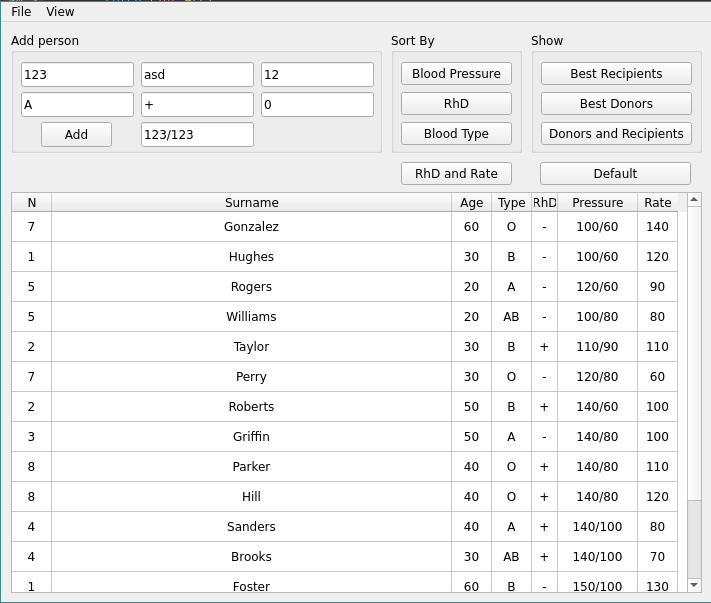
\includegraphics[scale=0.7]{4}
	\caption{Сортування записів за показником артеріального тиску}
\end{figure}

\subsection{Згрупувати людей за однаковими групами крові та однаковими резус факторами}
\begin{figure}[H]
	\centering
	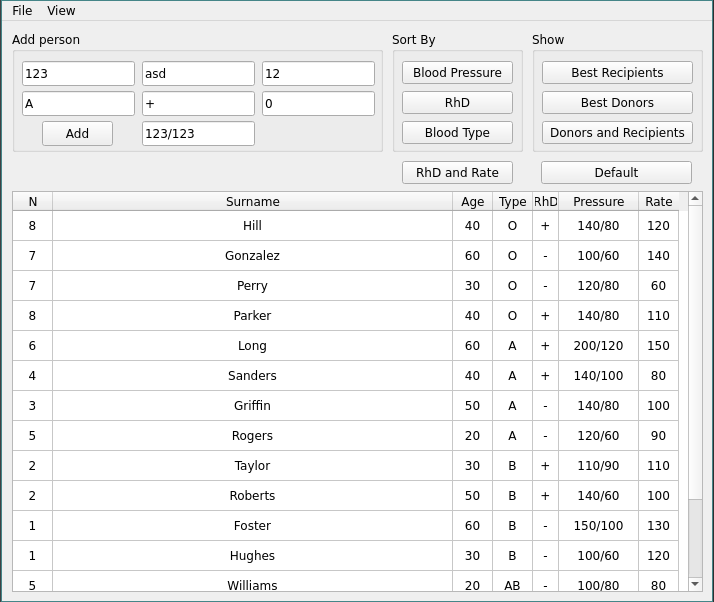
\includegraphics[scale=0.7]{5}
	\caption{Згрупувати людей за однаковими групами крові}
\end{figure}

\begin{figure}[H]
	\centering
	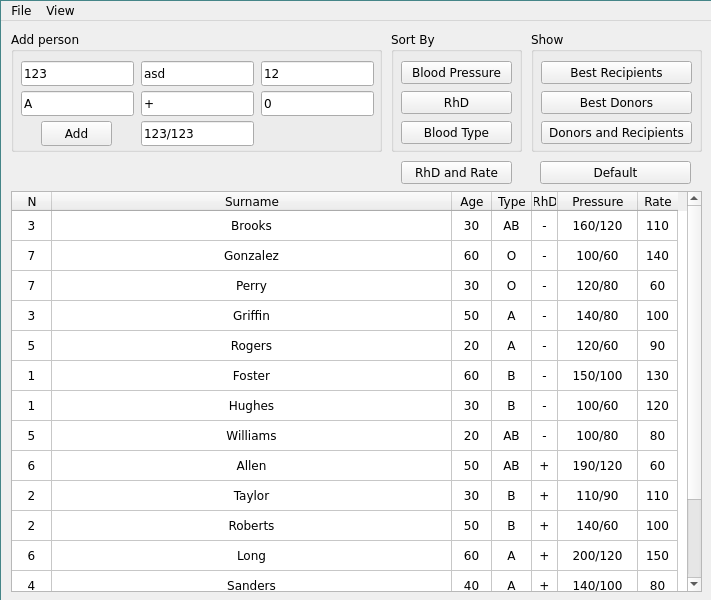
\includegraphics[scale=0.7]{6}
	\caption{Згрупувати людей за однаковими резус факторами}
\end{figure}

\subsection{Згрупувати людей за однаковими резус факторами та відсортувати кожну групу за показником пульсу}
\begin{figure}[H]
	\centering
	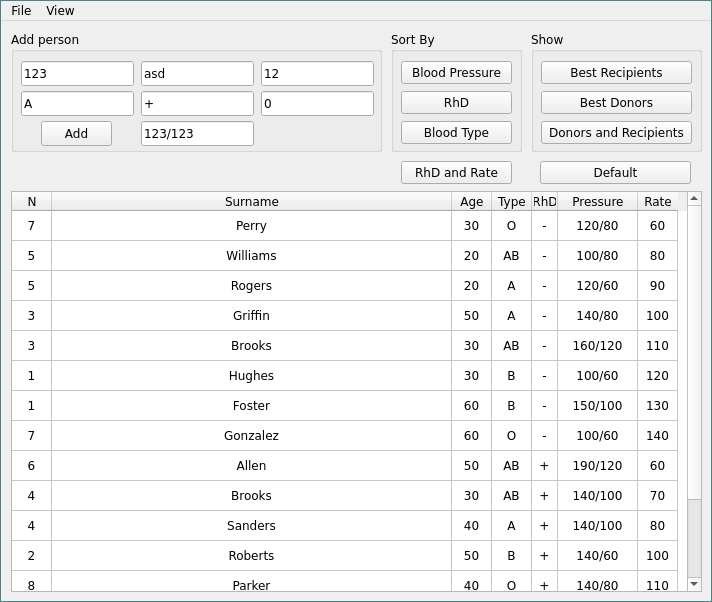
\includegraphics[scale=0.7]{7}
	\caption{Згрупувати людей за однаковими резус факторами та відсортувати кожну групу за показником пульсу}
\end{figure}

\subsection{Визначити людей, які є універсальними донорами, а які є універсальними реципієнтами та сформувати загальну таблицю донорів та реципієнтів}
\begin{figure}[H]
	\centering
	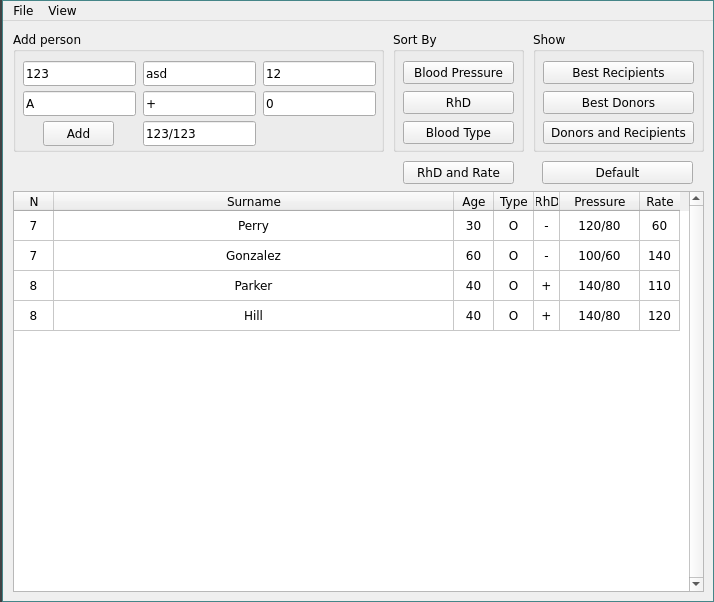
\includegraphics[scale=0.7]{8}
	\caption{Визначити людей, які є універсальними донорами}
\end{figure}

\begin{figure}[H]
	\centering
	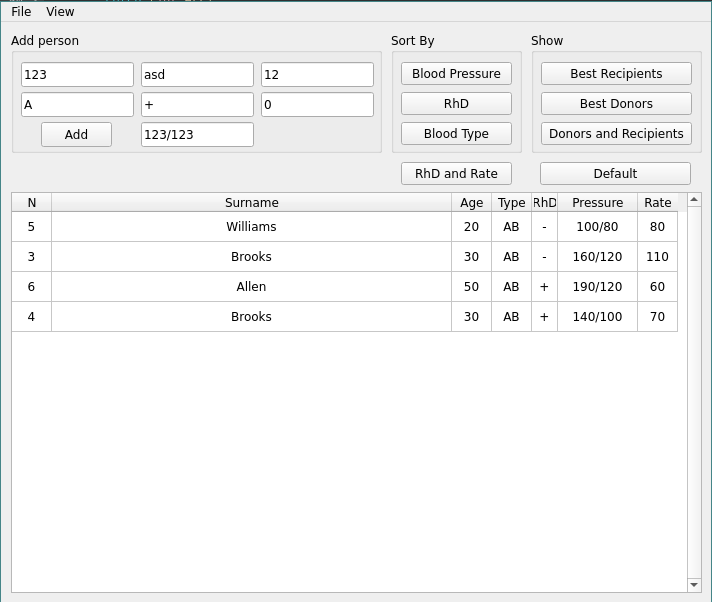
\includegraphics[scale=0.7]{9}
	\caption{Визначити людей, які є універсальними реципієнтами}
\end{figure}

\begin{figure}[H]
	\centering
	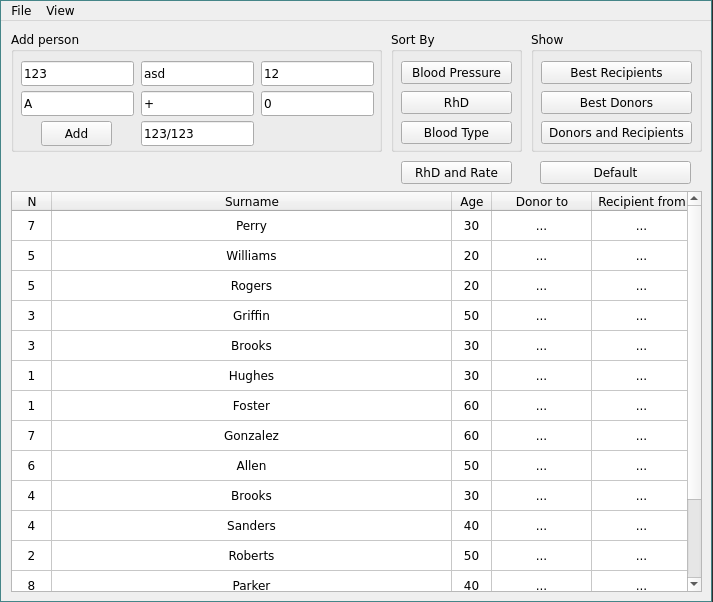
\includegraphics[scale=0.7]{10}
	\caption{Сформувати загальну таблицю донорів та реципієнтів}
\end{figure}

\subsection{Для вказаного показника вік  визначити пацієнтів з підвищеними показниками артеріального тиску та пульсу}
\begin{figure}[H]
	\centering
	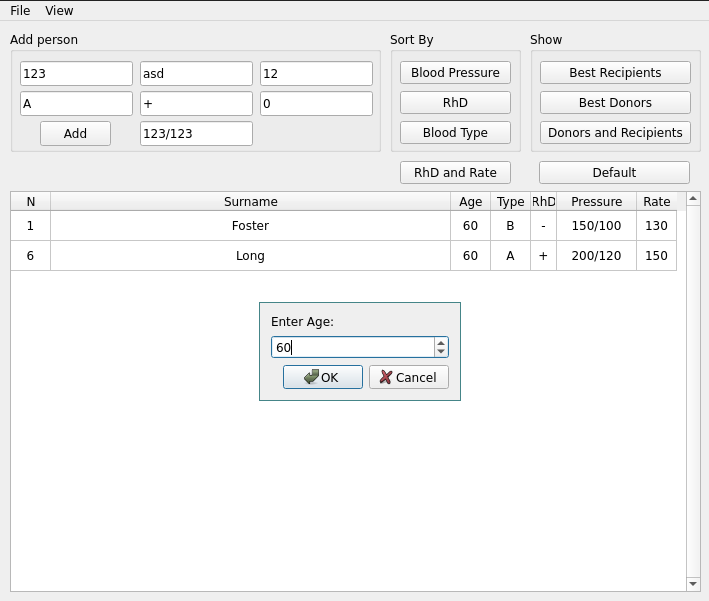
\includegraphics[scale=0.7]{11}
	\caption{Для вказаного показника вік  визначити пацієнтів з підвищеними показниками артеріального тиску та пульсу}
\end{figure}

\subsection{Всім пацієнтам з нормальним артеріальним тиском вивести повідомлення}
\begin{figure}[H]
	\centering
	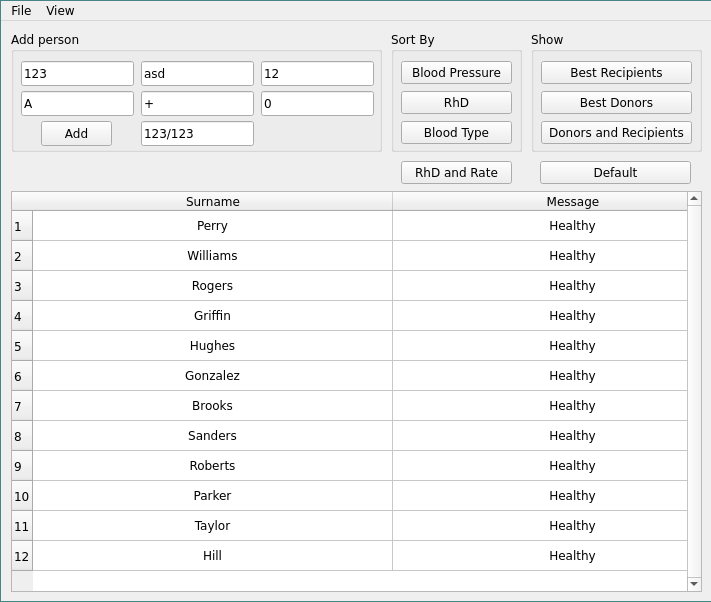
\includegraphics[scale=0.7]{12}
	\caption{Всім пацієнтам з нормальним артеріальним тиском вивести повідомлення}
\end{figure}

\section{Інструкція користувача та системні вимоги}
\subsection{Компоненти}
Програму розроблено на мовi програмування C++ у середовищi розробки QtCreator i може експлуатуватися пiд управлiнням сiмейства операцiйних систем GNU/Linux. Пiд час проектування пiдсистем вiдбувалося поєднання об’єктно-орiєнтованого пiдходу до програмування з процедурно орiєнтованим.

\subsection{Встановлення}
Програма не потребує встановлення, достатньо надати виконуваному файлу програми права на виконання та запустити його.
\subsection{Базові функції}
\begin{figure}[H]
	\centering
	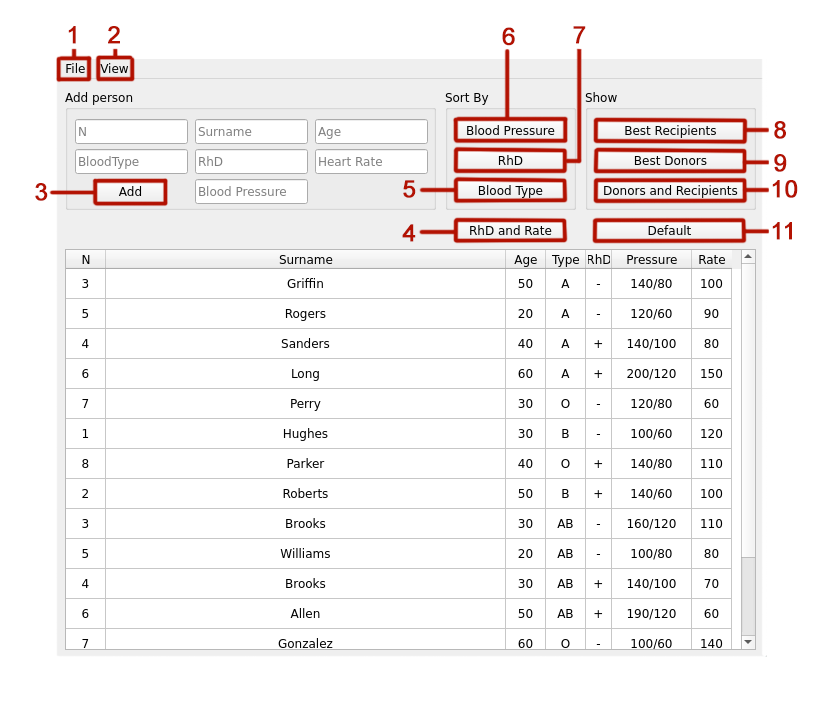
\includegraphics[scale=0.6]{13}
	\caption{Вигляд програми}
\end{figure}

\begin{enumerate}
	\item Діалог меню для роботи з файлами.
	\item Діалог меню для додаткових опцій сортування та перегляду.
	\item Кнопка для додавання нового користувача.
	\item Кнопка для групування за резус-фактором та сортування за пульсом.
	\item Кнопка для сортування за групою крові.
	\item Кнопка для сортування за артеріальним тиском.
	\item Кнопка для сортування за резус-фактором.
	\item Кнопка для перегляду таблиці універсальних реципієнтів.
	\item Кнопка для перегляду таблиці універсальних донорів.
	\item Кнопка для перегляду загальної таблиці донорів та реципієнтів.
	\item Кнопка для повернення таблиці до початкового стану.
\end{enumerate}

\subsection{Системні вимоги}
Для коректної роботи програми необхiдна користувацька машина з процесором не менше 1 GHz, оперативною пам’яттю не менше 512 Mb. Для експлуатацiї пакету пiд управлiнням сiмейства операцiйних систем GNU/Linux необхiдно встановити збiрку класiв Qt Framework 6.0.

\section{Опис виняткових ситуацій}
\subsection{Неправильні дані у полі для вводу під час додавання нового пацієнта}
\begin{figure}[H]
	\centering
	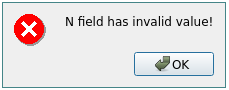
\includegraphics[scale=1]{14}
	\caption{Неправильні дані для поля N}
\end{figure}

\begin{figure}[H]
	\centering
	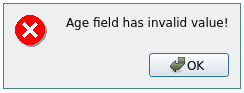
\includegraphics[scale=1]{15}
	\caption{Неправильні дані для поля Age}
\end{figure}

\begin{figure}[H]
	\centering
	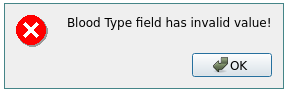
\includegraphics[scale=1]{16}
	\caption{Неправильні дані для поля Blood Type}
\end{figure}

\begin{figure}[H]
	\centering
	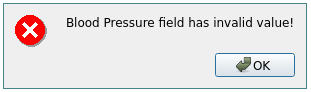
\includegraphics[scale=1]{17}
	\caption{Неправильні дані для поля Blood Pressure}
\end{figure}

\begin{figure}[H]
	\centering
	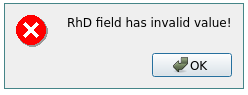
\includegraphics[scale=1]{18}
	\caption{Неправильні дані для поля RhD}
\end{figure}

\begin{figure}[H]
	\centering
	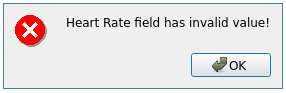
\includegraphics[scale=1]{19}
	\caption{Неправильні дані для поля Heart Rate}
\end{figure}

\subsection{Спроба відкрити файл з неправильними даними}
\begin{figure}[H]
	\centering
	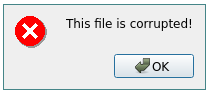
\includegraphics[scale=1]{21}
	\caption{Спроба відкрити файл з неправильними даними}
\end{figure}

\subsection{Обмежений діапазон даних для вводу}
\begin{figure}[H]
	\centering
	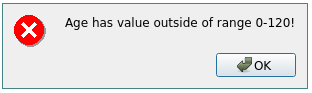
\includegraphics[scale=1]{20}
	\caption{Обмежений діапазон даних для поля Age}
\end{figure}

\begin{figure}[H]
	\centering
	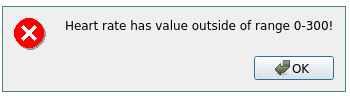
\includegraphics[scale=1]{22}
	\caption{Обмежений діапазон даних для поля Heart Rate}
\end{figure}

\section{Структура файлу вхідних даних}
Програма використовує класичний формат даних \textit{*.csv} (\textit{comma separated values}), тобто запис даних, де колонки розділяються комами, і кожен рядок знаходиться на новому рядку. 

\begin{figure}[H]
	\centering
	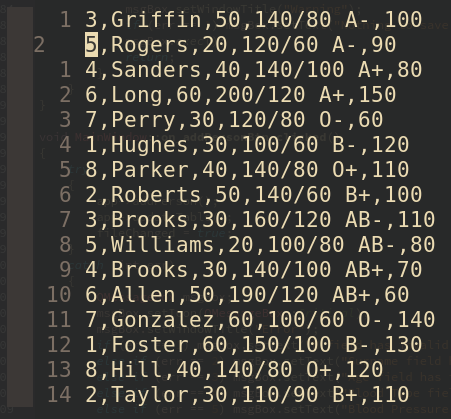
\includegraphics[scale=0.7]{23}
	\caption{Приклад файлу даних для програми}
\end{figure}

\section*{Висновки}
\addcontentsline{toc}{section}{Висновки}
Під час виконання курсової роботи я, закріпив теоретичні знання та практичні навички, набуті при вивченні дисципліни «Об'єктно-орієнтоване програмування».

У ході виконання курсової роботи я навчився самостійно працювати з технічною літературою, документацією, сучасними засобами розробки додатків засобами об'єктно орієнтованого програмування.

Я самостійно побудував програму <<Медична база пацієнтів>> у середовищі розробки QtCreator за допомогою фреймворку для десктопних додатків Qt 6.0 на мові C++ в об'єктно орієнтованому стилі.

\section*{Список використаної літератури}
\addcontentsline{toc}{section}{Список використаної літератури}
\begin{enumerate}
	\item \textit{https://vns.lpnu.ua/course/view.php?id=711} - курс Об'єктно Орієнтованого Програмування у віртуальному навчальному середовищі НУ <<ЛП>>.
	\item \textit{https://doc.qt.io/qt.html} - документація до фреймворку для десктопних додатків Qt 6.0.
	\item Кравець П.О. Обєктно-орієнтоване програмування. - Навчальний посібник. Львів: Видавництво Львівської політехніки, 2012. 624 с.
	\item Lee Zhi Eng, Qt5 C++ GUI Programming Cookbook - Second Edition, 2019
\end{enumerate}

\end{document}
